\documentclass[12pt]{article} % use larger type; default would be 10pt

\usepackage{pgfplots}
\usetikzlibrary{calc}
\usetikzlibrary{arrows}
\usetikzlibrary{patterns}
\usetikzlibrary{calc,intersections,through,backgrounds}
\usetikzlibrary{decorations.pathreplacing}
        \newcommand\degree[0]{^{\circ}}
        \newcommand\abs[1]{\left|#1\right|}

\title{Play with TikZ}
\author{Just Us}
%\date{} % Activate to display a given date or no date (if empty),
         % otherwise the current date is printed 

\begin{document}
\maketitle

\section{10.2 Polar Graphs }








fig10-3-1 parabola

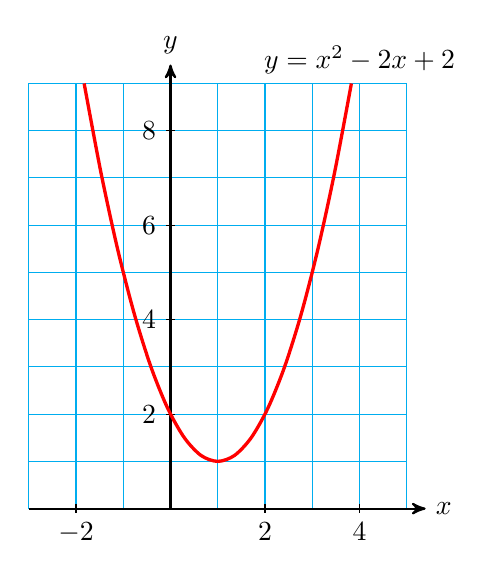
\begin{tikzpicture} [scale = .6]
\draw[cyan] (-3,0) grid (5,9);
\draw[black,thick,->,>=stealth'] (-3,0)--(5.4,0) node[right]{$x$};
\draw[black,thick,->,>=stealth'] (0,0)--(0, 9.4) node[above]{$y$};
\foreach \y in {2,4,6,8} {
\draw[black] (.1,\y) --++ (-.2,0) node[left]{$\y$};
}
\foreach \x in {-2,2,4} {
\draw[black] (\x,.1) --++ (0,-.2) node[below, yshift=-2, fill=white, inner sep=1]{$\x$};
}
\draw[domain={-2*sqrt(2)+1}:{2*sqrt(2)+1},smooth, samples=17,variable=\x,red,very thick] plot (\x,{(\x)^2-2*\x+2)});
\node[above] at (4,9) {$y=x^2-2x+2$};
\end{tikzpicture}
\newline




exam10-3-7 conjugates in complex plane

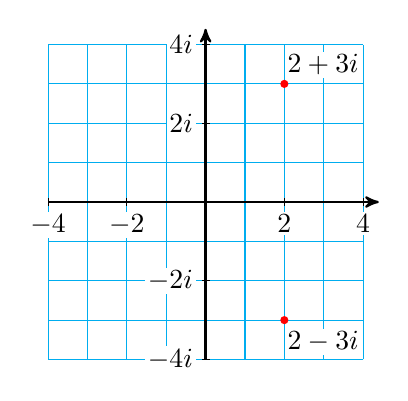
\begin{tikzpicture} [scale = .5]
\draw[cyan] (-4,-4) grid (4,4);
\draw[black,thick,->,>=stealth'] (-4,0)--(4.4,0);
\draw[black,thick,->,>=stealth'] (0,-4)--(0, 4.4);
\foreach \y in {2,4} {
\draw[black] (.1,\y) --++ (-.2,0) node[left, xshift=-2, fill=white, inner sep=1]{$\y i$};
\draw[black] (.1,-\y) --++ (-.2,0) node[left, xshift=-2, fill=white, inner sep=1]{$-\y i$};
}
\foreach \x in {2,4} {
\draw[black] (\x,.1) --++ (0,-.2) node[below, yshift=-2, fill=white, inner sep=1]{$\x$};
\draw[black] (-\x,.1) --++ (0,-.2) node[below, yshift=-2, fill=white, inner sep=1]{$-\x$};
}
\draw[red, fill=red] (2,3) circle (2.5pt) node[above right, yshift=2, fill=white, inner sep=1, text=black] {$2+3i$};
\draw[red, fill=red] (2,-3) circle (2.5pt) node[below right, yshift=-3, fill=white, inner sep=1, text=black] {$2-3i$};
\end{tikzpicture}
\newline

exer10-3-7 conjugates in complex plane

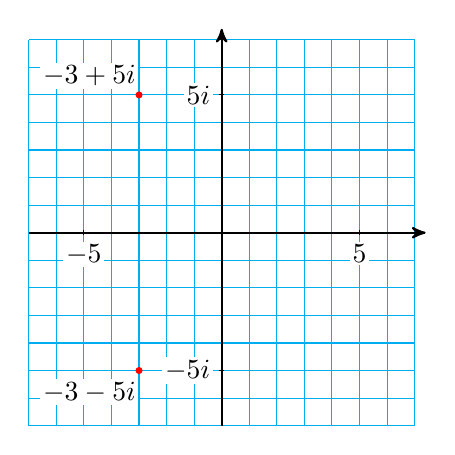
\begin{tikzpicture} [scale = .35]
\draw[cyan] (-7,-7) grid (7,7);
\draw[black,thick,->,>=stealth'] (-7,0)--(7.4,0);
\draw[black,thick,->,>=stealth'] (0,-7)--(0, 7.4);
\foreach \y in {5} {
\draw[black] (.1,\y) --++ (-.2,0) node[left, xshift=-2, fill=white, inner sep=1]{$\y i$};
\draw[black] (.1,-\y) --++ (-.2,0) node[left, xshift=-2, fill=white, inner sep=1]{$-\y i$};
}
\foreach \x in {5} {
\draw[black] (\x,.1) --++ (0,-.2) node[below, yshift=-2, fill=white, inner sep=1]{$\x$};
\draw[black] (-\x,.1) --++ (0,-.2) node[below, yshift=-2, fill=white, inner sep=1]{$-\x$};
}
\draw[red, fill=red] (-3,5) circle (3pt) node[above left, yshift=2, fill=white, inner sep=1, text=black] {$-3+5i$};
\draw[red, fill=red] (-3,-5) circle (3pt) node[below left, yshift=-3, fill=white, inner sep=1, text=black] {$-3-5i$};
\end{tikzpicture}
\newline

exam10-3-8 circle

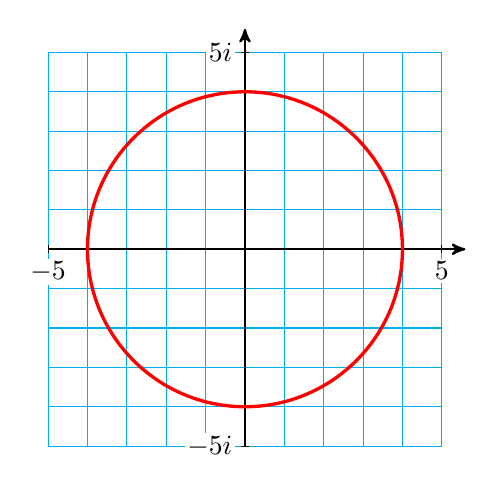
\begin{tikzpicture} [scale = .5]
\draw[cyan] (-5,-5) grid (5,5);
\draw[black,thick,->,>=stealth'] (-5,0)--(5.6,0);
\draw[black,thick,->,>=stealth'] (0,-5)--(0, 5.6);
\foreach \y in {5} {
\draw[black] (.1,\y) --++ (-.2,0) node[left, xshift=-2, fill=white, inner sep=1]{$\y i$};
\draw[black] (.1,-\y) --++ (-.2,0) node[left, xshift=-2, fill=white, inner sep=1]{$-\y i$};
}
\foreach \x in {5} {
\draw[black] (\x,.1) --++ (0,-.2) node[below, yshift=-2, fill=white, inner sep=1]{$\x$};
\draw[black] (-\x,.1) --++ (0,-.2) node[below, yshift=-2, fill=white, inner sep=1]{$-\x$};
}
\draw[red, very thick] (0,0) circle (4 cm);
\end{tikzpicture}
\newline

fig10-3-2 vectors 

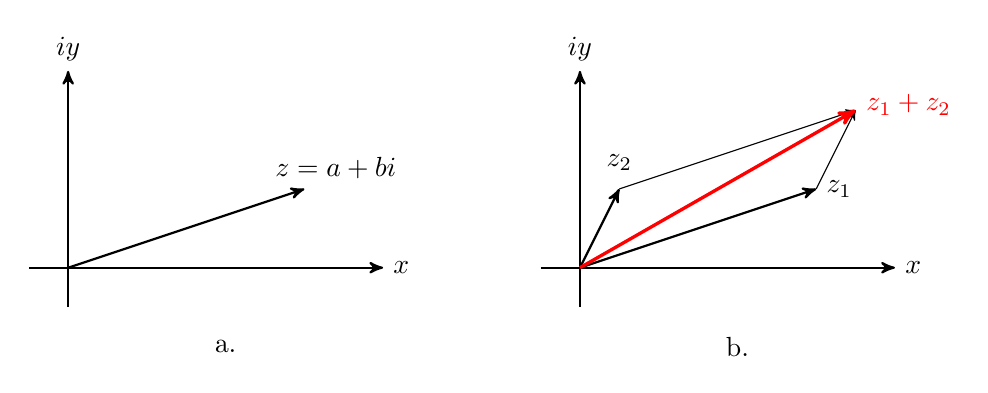
\begin{tikzpicture} 
\coordinate (O) at (0,0);
\coordinate (z) at (3,1);
\draw[black,thick,->,>=stealth'] (-.5,0)--++(4.5,0) node[right]{$x$};
\draw[black,thick,->,>=stealth'] (0,-.5)--++(0, 3) node[above]{$iy$};;
\draw[black, thick, ->, >=stealth'] (O) -- ++(z) node[above right, xshift=-.5cm]{$z=a+b i$};
\node at (2,-1){a.};
%second picture
\def\del{6.5};
\coordinate (O) at (\del,0);
\coordinate (z2) at (.5,1);
\draw[black,thick,->,>=stealth'] (O)++(-.5,0)--++(4.5,0) node[right]{$x$};
\draw[black,thick,->,>=stealth'] (O)++(0,-.5)--++(0, 3) node[above]{$iy$};;
\draw[black, thick, ->, >=stealth'] (O) -- ++(z) node[right]{$z_1$};
\draw[black,  ->, >=stealth'] (O)++(z2) -- ++(z);
\draw[black, thick, ->, >=stealth'] (O) -- ++(z2) node[above , yshift=.1cm]{$z_2$};
\draw[black, ->, >=stealth'] (O)++(z) -- ++(z2);
\draw[red, very thick, ->, >=stealth'] (O) -- ++($ (z)+(z2)$) node[above right, yshift=-.2cm]{$z_1 + z_2$};
\node at ({\del+2},-1){b.};

\end{tikzpicture}
\newline

exam10-3-9. vectors 

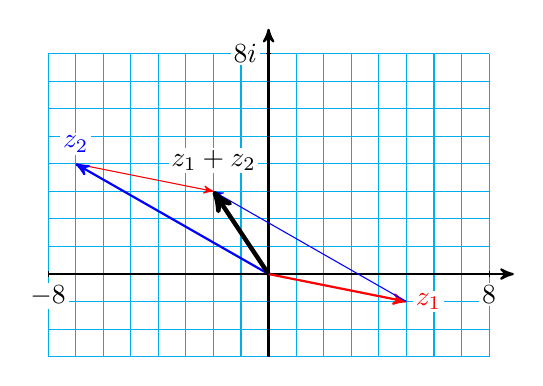
\begin{tikzpicture} [scale=.35]
\draw[cyan] (-8,-3) grid (8,8);
\foreach \y in {8} {
\draw[black] (.1,\y) --++ (-.2,0) node[left, xshift=-2, fill=white, inner sep=1]{$\y i$};
}
\foreach \x in {-8,8} {
\draw[black] (\x,.1) --++ (0,-.2) node[below, yshift=-2, fill=white, inner sep=1]{$\x$};
}
\coordinate (O) at (0,0);
\coordinate (z) at (5,-1);
\coordinate (z2) at (-7,4);
\draw[black,thick,->,>=stealth'] (-8,0)--++(16.9,0);
\draw[black,thick,->,>=stealth'] (0,-3)--++(0, 11.9);
\draw[red, thick, ->, >=stealth'] (O) -- ++(z) node[right, xshift=2, fill=white, inner sep=1]{$z_1$};
\draw[red,  ->, >=stealth'] (z2) -- ++(z);
\draw[blue, thick, ->, >=stealth'] (O) -- ++(z2) node[above , yshift=.1cm, fill=white, inner sep=1]{$z_2$};
\draw[blue, ->, >=stealth'] (O)++(z) -- ++(z2);
\draw[black, ultra thick, ->, >=stealth'] (O) -- ++($ (z)+(z2)$) node[above , yshift=.2cm, fill=white, inner sep=1]{$z_1+z_2$};
\end{tikzpicture}
\newline

exer10-3-9 vectors 

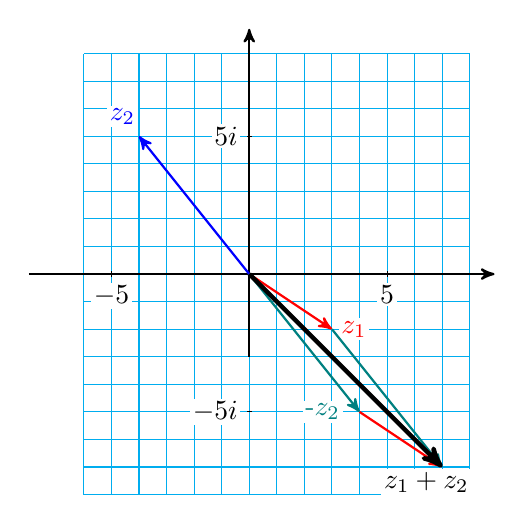
\begin{tikzpicture} [scale=.35]
\draw[cyan] (-6,-8) grid (8,8);
\foreach \y in {-5,5} {
\draw[black] (.1,\y) --++ (-.2,0) node[left, xshift=-2, fill=white, inner sep=1]{$\y i$};
}
\foreach \x in {-5,5} {
\draw[black] (\x,.1) --++ (0,-.2) node[below, yshift=-2, fill=white, inner sep=1]{$\x$};
}
\coordinate (O) at (0,0);
\coordinate (z) at (3,-2);
\coordinate (z2) at (-4,5);
\coordinate (nz2) at (4,-5);
\draw[black,thick,->,>=stealth'] (-8,0)--++(16.9,0);
\draw[black,thick,->,>=stealth'] (0,-3)--++(0, 11.9);
\draw[red, thick, ->, >=stealth'] (O) -- ++(z) node[right, xshift=2, fill=white, inner sep=1]{$z_1$};
\draw[red,thick,  ->, >=stealth'] (nz2) -- ++(z);
\draw[blue, thick, ->, >=stealth'] (O) -- ++(z2) node[above left, yshift=.1cm, fill=white, inner sep=1]{$z_2$};
\draw[teal,thick, ->, >=stealth'] (O) -- ++(nz2) node[left, xshift=-.2cm, fill=white, inner sep=1]{-$z_2$};
\draw[teal,thick, ->, >=stealth'] (z) -- ++(nz2);
\draw[black, ultra thick, ->, >=stealth'] (O) -- ++($ (z)+(nz2)$) node[below , xshift=-.2cm, fill=white, inner sep=1]{$z_1+z_2$};
\end{tikzpicture}
\newline



fig10-3-3 quartic

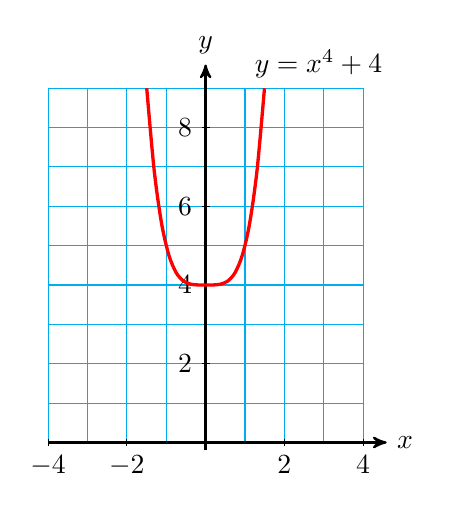
\begin{tikzpicture} [scale = .5]
\draw[cyan] (-4,0) grid (4,9);
\draw[black,thick,->,>=stealth'] (-4,0)--(4.6,0) node[right]{$x$};
\draw[black,thick,->,>=stealth'] (0,-.2)--(0, 9.6) node[above]{$y$};
\foreach \y in {2,4,6,8} {
\draw[black] (.1,\y) --++ (-.2,0) node[left]{$\y$};
}
\foreach \x in {-4,-2,2,4} {
\draw[black] (\x,.1) --++ (0,-.2) node[below, yshift=-2, fill=white, inner sep=1]{$\x$};
}
\draw[domain={-(5)^(1/4)}:{(5)^(1/4)},smooth, samples=17,variable=\x,red,very thick] plot (\x,{(\x)^4+4)});
\node[above right] at (1,9) {$y=x^4 +4$};
\end{tikzpicture}
\newline

hp10-3-47ans conjugates in complex plane

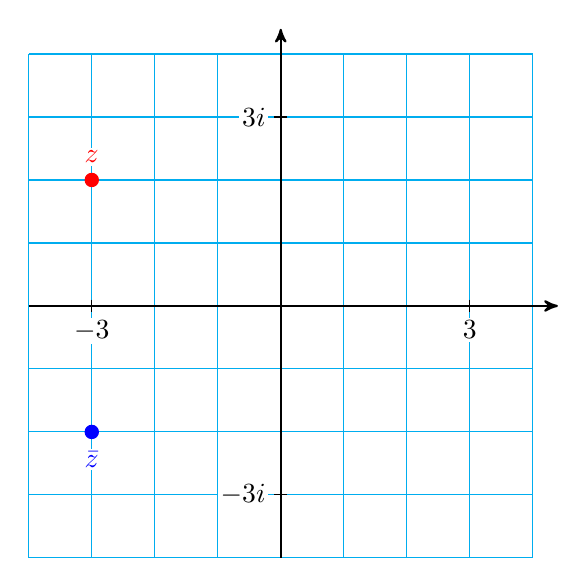
\begin{tikzpicture} [scale = .8]
\draw[cyan] (-4,-4) grid (4,4);
\draw[black,thick,->,>=stealth'] (-4,0)--(4.4,0);
\draw[black,thick,->,>=stealth'] (0,-4)--(0, 4.4);
\foreach \y in {3} {
\draw[black] (.1,\y) --++ (-.2,0) node[left, xshift=-2, fill=white, inner sep=1]{$\y i$};
\draw[black] (.1,-\y) --++ (-.2,0) node[left, xshift=-2, fill=white, inner sep=1]{$-\y i$};
}
\foreach \x in {3} {
\draw[black] (\x,.1) --++ (0,-.2) node[below, yshift=-2, fill=white, inner sep=1]{$\x$};
\draw[black] (-\x,.1) --++ (0,-.2) node[below, yshift=-2, fill=white, inner sep=1]{$-\x$};
}
\draw[red, fill=red] (-3,2) circle (3pt) node[above , yshift=5, fill=white, inner sep=1] {$z$};
\draw[blue, fill=blue] (-3,-2) circle (3pt) node[below , yshift=-6, fill=white, inner sep=1] {$\bar{z}$};
\end{tikzpicture}
\newline

hp10-3-49ans conjugates in complex plane

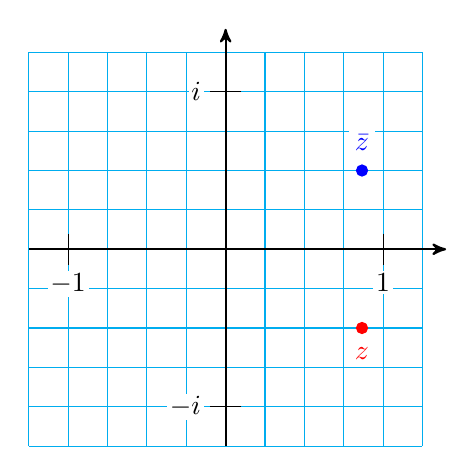
\begin{tikzpicture} [scale = 2]
\draw[cyan] (-5/4,-5/4) grid[step=1/4] (5/4,5/4);
\draw[black,thick,->,>=stealth'] (-1.25,0)--(1.4,0);
\draw[black,thick,->,>=stealth'] (0,-1.25)--(0, 1.4);
\foreach \y in {1} {
\draw[black] (.1,\y) --++ (-.2,0) node[left, xshift=-2, fill=white, inner sep=1]{$ i$};
\draw[black] (.1,-\y) --++ (-.2,0) node[left, xshift=-2, fill=white, inner sep=1]{$-i$};
}
\foreach \x in {1} {
\draw[black] (\x,.1) --++ (0,-.2) node[below, yshift=-2, fill=white, inner sep=1]{$\x$};
\draw[black] (-\x,.1) --++ (0,-.2) node[below, yshift=-2, fill=white, inner sep=1]{$-\x$};
}
\draw[red, fill=red] (-30:1) circle (1pt) node[below , yshift=-6, fill=white, inner sep=1] {$z$};
\draw[blue, fill=blue] (30:1) circle (1pt) node[above , yshift=5, fill=white, inner sep=2] {$\bar{z}$};
\end{tikzpicture}
\newline

hp10-3-51ans disk in complex plane

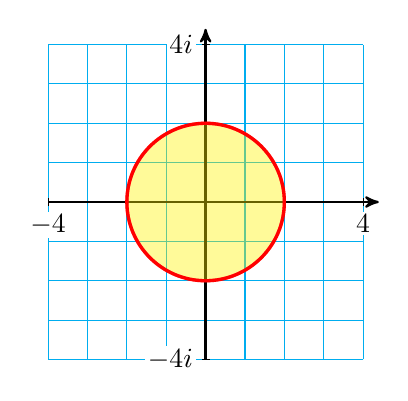
\begin{tikzpicture} [scale = .5]
\draw[cyan] (-4,-4) grid (4,4);
\draw[black,thick,->,>=stealth'] (-4,0)--(4.4,0);
\draw[black,thick,->,>=stealth'] (0,-4)--(0, 4.4);
\foreach \y in {4} {
\draw[black] (.1,\y) --++ (-.2,0) node[left, xshift=-2, fill=white, inner sep=1]{$\y i$};
\draw[black] (.1,-\y) --++ (-.2,0) node[left, xshift=-2, fill=white, inner sep=1]{$-\y i$};
}
\foreach \x in {4} {
\draw[black] (\x,.1) --++ (0,-.2) node[below, yshift=-2, fill=white, inner sep=1]{$\x$};
\draw[black] (-\x,.1) --++ (0,-.2) node[below, yshift=-2, fill=white, inner sep=1]{$-\x$};
}
\draw[red, very thick, fill=yellow, opacity=.4] (0,0) circle (2cm);
\draw[red, very thick] (0,0) circle (2cm);
\end{tikzpicture}
\newline

hp10-3-53ans half-plane

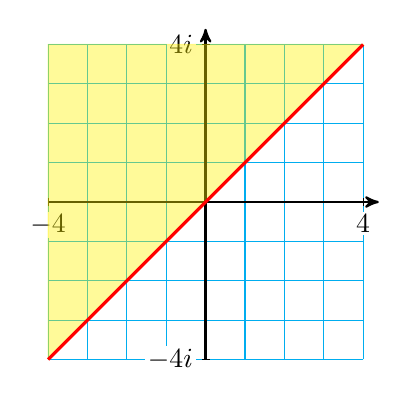
\begin{tikzpicture} [scale = .5]
\draw[cyan] (-4,-4) grid (4,4);
\draw[black,thick,->,>=stealth'] (-4,0)--(4.4,0);
\draw[black,thick,->,>=stealth'] (0,-4)--(0, 4.4);
\foreach \y in {4} {
\draw[black] (.1,\y) --++ (-.2,0) node[left, xshift=-2, fill=white, inner sep=1]{$\y i$};
\draw[black] (.1,-\y) --++ (-.2,0) node[left, xshift=-2, fill=white, inner sep=1]{$-\y i$};
}
\foreach \x in {4} {
\draw[black] (\x,.1) --++ (0,-.2) node[below, yshift=-2, fill=white, inner sep=1]{$\x$};
\draw[black] (-\x,.1) --++ (0,-.2) node[below, yshift=-2, fill=white, inner sep=1]{$-\x$};
}
\draw[yellow,fill=yellow, opacity=.4] (-4,-4) -- (4,4)--(-4,4)--(-4,-4);
\draw[red, very thick] (-4,-4) -- (4,4);
\end{tikzpicture}
\newline

hp10-3-53ans half-plane

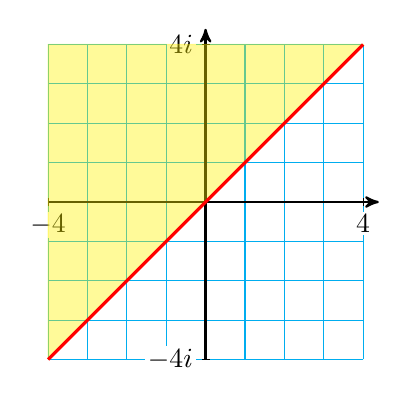
\begin{tikzpicture} [scale = .5]
\draw[cyan] (-4,-4) grid (4,4);
\draw[black,thick,->,>=stealth'] (-4,0)--(4.4,0);
\draw[black,thick,->,>=stealth'] (0,-4)--(0, 4.4);
\foreach \y in {4} {
\draw[black] (.1,\y) --++ (-.2,0) node[left, xshift=-2, fill=white, inner sep=1]{$\y i$};
\draw[black] (.1,-\y) --++ (-.2,0) node[left, xshift=-2, fill=white, inner sep=1]{$-\y i$};
}
\foreach \x in {4} {
\draw[black] (\x,.1) --++ (0,-.2) node[below, yshift=-2, fill=white, inner sep=1]{$\x$};
\draw[black] (-\x,.1) --++ (0,-.2) node[below, yshift=-2, fill=white, inner sep=1]{$-\x$};
}
\draw[yellow,fill=yellow, opacity=.4] (-4,-4) -- (4,4)--(-4,4)--(-4,-4);
\draw[red, very thick] (-4,-4) -- (4,4);
\end{tikzpicture}
\newline

hp10-3-55ans vectors 

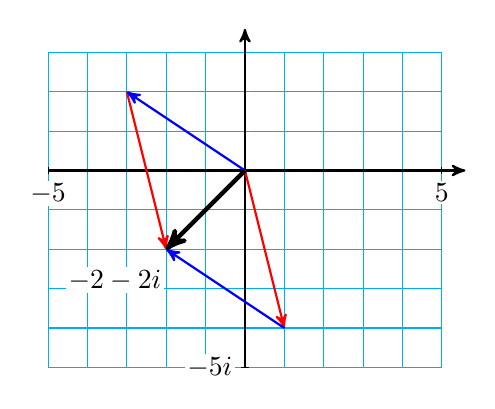
\begin{tikzpicture} [scale=.5]
\draw[cyan] (-5,-5) grid (5,3);
\foreach \y in {-5} {
\draw[black] (.1,\y) --++ (-.2,0) node[left, xshift=-2, fill=white, inner sep=1]{$\y i$};
}
\foreach \x in {-5,5} {
\draw[black] (\x,.1) --++ (0,-.2) node[below, yshift=-2, fill=white, inner sep=1]{$\x$};
}
\coordinate (O) at (0,0);
\coordinate (z) at (1,-4);
\coordinate (z2) at (-3,2);
\draw[black,thick,->,>=stealth'] (-5,0)--(5.6,0);
\draw[black,thick,->,>=stealth'] (0,-5)--(0, 3.6);
\draw[red, thick, ->, >=stealth'] (O) -- ++(z);
\draw[red, thick,  ->, >=stealth'] (z2) -- ++(z);
\draw[blue, thick, ->, >=stealth'] (O) -- ++(z2);
\draw[blue, thick, ->, >=stealth'] (O)++(z) -- ++(z2);
\draw[black, ultra thick, ->, >=stealth'] (O) -- ++($ (z)+(z2)$) node[below left, yshift=-.2cm, fill=white, inner sep=1]{$-2 - 2i$};
\end{tikzpicture}
\newline

hp10-3-57ans vectors 

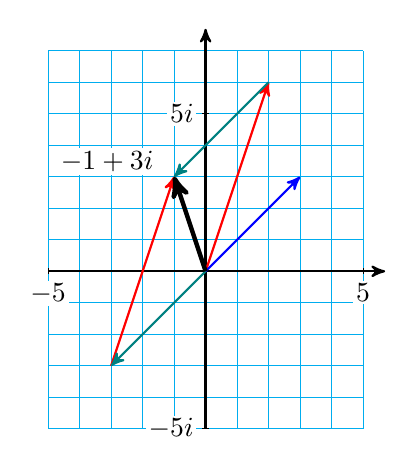
\begin{tikzpicture} [scale=.4]
\draw[cyan] (-5,-5) grid (5,7);
\foreach \y in {-5,5} {
\draw[black] (.1,\y) --++ (-.2,0) node[left, xshift=-2, fill=white, inner sep=1]{$\y i$};
}
\foreach \x in {-5,5} {
\draw[black] (\x,.1) --++ (0,-.2) node[below, yshift=-2, fill=white, inner sep=1]{$\x$};
}
\coordinate (O) at (0,0);
\coordinate (z) at (2,6);
\coordinate (z2) at (3,3);
\coordinate (nz2) at (-3,-3);
\draw[black,thick,->,>=stealth'] (-5,0)--(5.7,0);
\draw[black,thick,->,>=stealth'] (0,-5)--(0, 7.7);
\draw[red, thick, ->, >=stealth'] (O) -- ++(z);
\draw[red,thick,  ->, >=stealth'] (nz2) -- ++(z);
\draw[blue, thick, ->, >=stealth'] (O) -- ++(z2);
\draw[teal,thick, ->, >=stealth'] (O) -- ++(nz2);
\draw[teal,thick, ->, >=stealth'] (z) -- ++(nz2);
\draw[black, ultra thick, ->, >=stealth'] (O) -- ++($ (z)+(nz2)$) node[above left, xshift=-.2cm, fill=white, inner sep=1]{$-1+3i$};
\end{tikzpicture}
\newline






\end{document}
